% \tikzexternaldisable

\tikzsetnextfilename{fig-cubic-string}
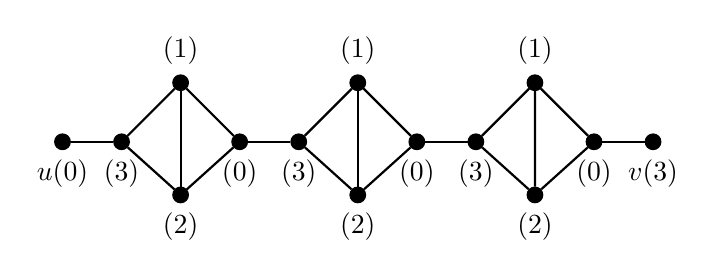
\begin{tikzpicture}[scale=0.75,
    vertex/.style={circle, draw, fill=black, inner sep=2pt},
    redvertex/.style={circle, draw, fill=red, inner sep=2pt},
    edge/.style={draw, thick}
]

% (mismo dibujo)
\node[vertex, label=below:$u (0)$] (u) at (0,0) {};
\node[vertex,label=below:$(3)$] (a1) at (1,0) {};
\draw[edge] (u) -- (a1);

\node[vertex, label=above:$(1)$] (t1) at (2,1) {};
\node[vertex,label=below:$(2)$] (b1) at (2,-0.9) {};
\node[vertex,label=below:$(0)$] (c1) at (3,0) {};
\draw[edge] (a1) -- (t1);
\draw[edge] (a1) -- (b1);
\draw[edge] (b1) -- (c1);
\draw[edge] (c1) -- (t1);
\draw[edge] (t1) -- (b1);

\node[vertex,label=below:$(3)$] (a2) at (4,0) {};
\draw[edge] (c1) -- (a2);

\node[vertex, label=above:$(1)$] (t2) at (5,1) {};
\node[vertex,label=below:$(2)$] (b2) at (5,-0.9) {};
\node[vertex,label=below:$(0)$] (c2) at (6,0) {};
\draw[edge] (a2) -- (t2);
\draw[edge] (a2) -- (b2);
\draw[edge] (b2) -- (c2);
\draw[edge] (c2) -- (t2);
\draw[edge] (t2) -- (b2);

\node[vertex,label=below:$(3)$] (a3) at (7,0) {};
\draw[edge] (c2) -- (a3);

\node[vertex, label=above:$(1)$] (t3) at (8,1) {};
\node[vertex, label=below:$(2)$] (b3) at (8,-0.9) {};
\node[vertex, label=below:$(0)$] (c3) at (9,0) {};
\draw[edge] (a3) -- (t3);
\draw[edge] (a3) -- (b3);
\draw[edge] (b3) -- (c3);
\draw[edge] (c3) -- (t3);
\draw[edge] (t3) -- (b3);

\node[vertex, label=below:$v (3)$] (v) at (10,0) {};
\draw[edge] (c3) -- (v);
\end{tikzpicture}
% \caption{$ $.}